\begin{frame}[parent={cmap:jabuti-gui},hasnext=true,hasprev=true]
\frametitle{Graphical user interface}
\framesubtitle{Main functionalities - Tools}
\label{concept:main-functionalities:tools}

\vfill
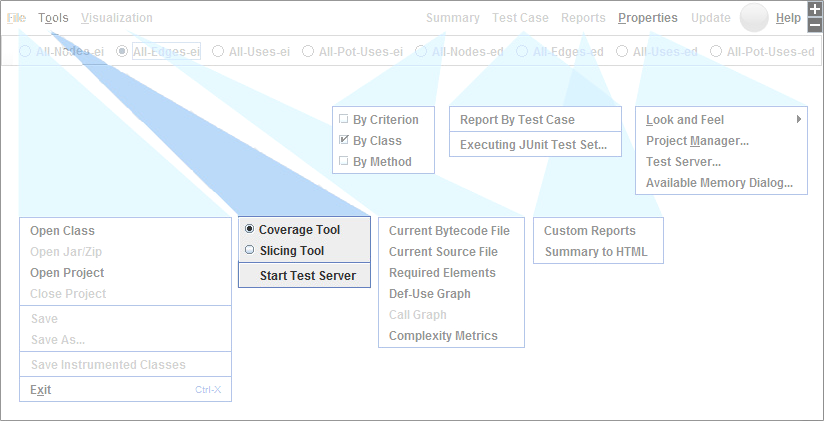
\includegraphics[width=\textwidth,clip]{resources/JaBUTi/JaBUTi-GUI/JaBUTi-GUI-Tools/JaBUTi-GUI-Tools-Expanded}
\vfill
\end{frame}


\begin{frame}
\frametitle{Main functionalities}
\framesubtitle{Tools Menu}
\label{concept:tools-menu}
\label{concept:coverage-tool}
\label{concept:slicing-tool}
\label{concept:start-test-server}

\begin{block}{Tools}
The \highlight{Tools} menu provides access to JaBUTi's tools.
\end{block}

\begin{columns}[t]
\column{.5\textwidth}
\begin{block}{Tools}
\begin{itemize}
	\item \highlight{Coverage Tool}: enables JaBUTi's coverage tool.
	\item \highlight{Slicing Tool}: enables JaBUTi's slicing tool.
	\item \highlight{Start Test Server}: starts the test server for mobile
	devices.
\end{itemize}
\end{block}
\column{.5\textwidth}
\begin{block}{Demo}
	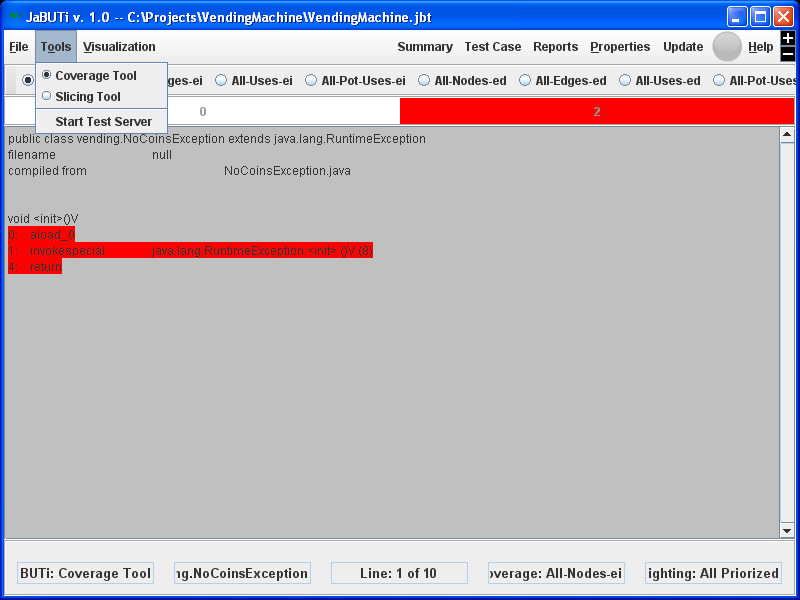
\includegraphics[scale=.6,clip,trim=0 200 360 0]{resources/JaBUTi/JaBUTi-GUI/JaBUTi-GUI-Tools/JaBUTi-GUI-Tools}
\end{block}
\end{columns}

\end{frame}